% Figure S1 — per-iteration timing (Damped-NP order=5 vs ISI)
% Suggested Overleaf path: "S1 Figure/figure_s1.tex"
% Upload the PDF "order5_np_damped_isi_per_iteration_time.pdf" to the same
% project and adjust the \includegraphics path if needed.
\begin{figure}[htbp]
\centering
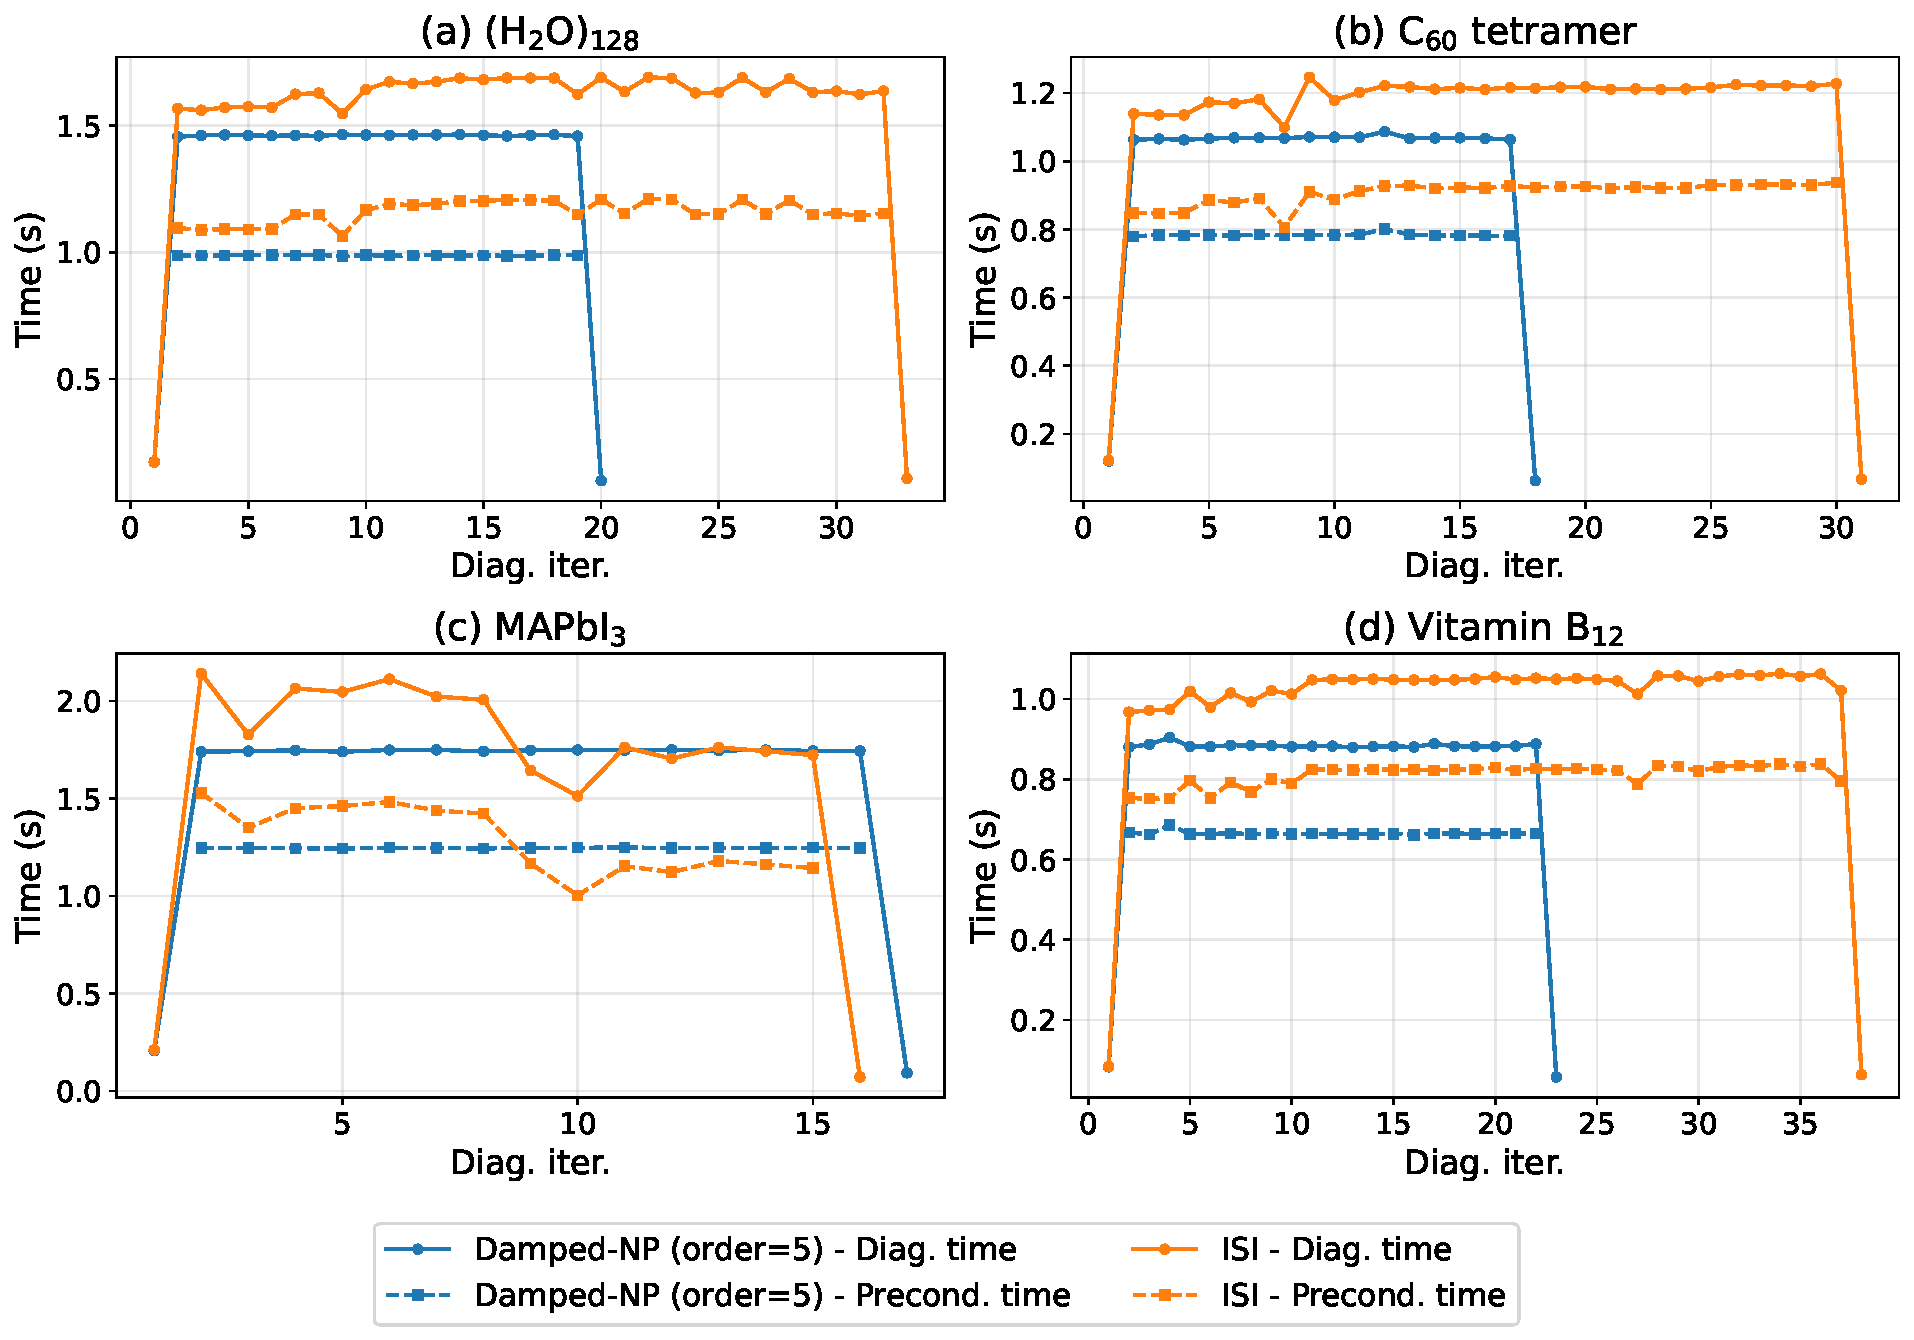
\includegraphics[width=\linewidth]{order5_np_damped_isi_per_iteration_time.pdf}
\caption{%
Per-iteration cost of the Damped-NP (order $=5$) and ISI preconditioners
under \emph{fixed-Hamiltonian} diagonalization \emph{without the locking
scheme}. Diagonalization time (solid lines, circles) and preconditioning
time (dashed lines, squares) are shown versus the outer diagonalization
iteration index for
(a)~$(\mathrm{H_2O})_{128}$,
(b)~$\mathrm{C}_{60}$ tetramer,
(c)~$\mathrm{MAPbI}_{3}$, and
(d)~Vitamin~$\mathrm{B}_{12}$.
The Hamiltonian is held fixed across iterations and the locking scheme is
disabled, so every outer step operates on the full subspace and the
per-iteration cost reflects the intrinsic behavior of each preconditioner.
Colors denote the preconditioner (blue: Damped-NP (order $=5$); orange:
ISI) and line styles denote the timed quantity (solid: diagonalization
time; dashed: preconditioning time). The first iteration carries no
preconditioning step and the last iteration is a partial/convergence step,
which appear as the dips at the curve endpoints. Across all four systems
Damped-NP shows an essentially constant per-iteration cost, whereas ISI
exhibits a noticeably larger variation driven by its inner iterative solve
(see Table~\ref{tab:s2_per_iter_std}).%
}
\label{fig:s1_per_iter_time}
\end{figure}
